\section{Pruebas de independencia}
\label{sec:independencia}

\subsection{Regresando a nuestro ejemplo...}
El número de grados de libertad es el número de categorías menos uno.  En nuestro ejemplo $\nu = 2-1 =1.$  Supongamos un nivel de significación $\beta=0.05.$


\begin{figure}
	\centering
	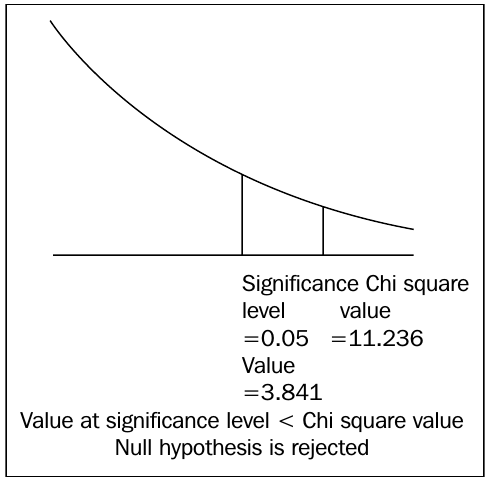
\includegraphics[height=5cm,keepaspectratio=true]{./images/kum0407.png}
	% kum0407.png: 0x0 pixel, 300dpi, 0.00x0.00 cm, bb=
	\caption{La hipótesis nula se rechaza porque el valor del estadístico $\chi^2$ al nivel de significación es menor que el valor del estadístico.}
	\label{fig:3.9.2}
\end{figure}


Examinemos otros ejemplo donde queremos demostrar que el género de un estudiante y las materias que escoge son independientes.


Supongamos que un grupo de estudiantes, la siguiente tabla representa el número de hombres y mujeres que toman matemáticas, arte y comercio como sus materias principales.


\begin{center}
	\begin{tabular}{|l|l|l|l|l|}\hline
		& Matemáticas & Artes & Comercio & Total\\\hline
		Hombres & 68 & 52 & 90 & 210\\\hline
		Mujeres & 28 & 37 & 35 & 100\\\hline
		Total & 106 & 89 & 125 & 310\\\hline
	\end{tabular}
\end{center}



Si en la elección de las materias, no fuera relevante el género, entonces el número esperado de hombres y mujeres tomando diferentes materias sería
\begin{center}
	\begin{tabular}{|l|l|l|l|l|}\hline
		& Matemáticas & Arte & Comercio & Total\\\hline
		Hombres & 71.81 & 60.29 & 84.90 & 210\\\hline
		Mujeres & 34.19 & 28.71 & 40.10 & 100\\\hline
		Total & 106 & 89 & 125 & 310\\\hline
	\end{tabular}
\end{center}

Los valores esperados se calculan como $E_{ij} = \frac{(\text{Total fila}_i)(\text{Total columna}_j)}{\text{Total general}}$:
\begin{align}
	E_{11} &= \frac{210 \times 106}{310} = 71.81 \\
	E_{12} &= \frac{210 \times 89}{310} = 60.29 \\
	E_{13} &= \frac{210 \times 125}{310} = 84.90 \\
	E_{21} &= \frac{100 \times 106}{310} = 34.19 \\
	E_{22} &= \frac{100 \times 89}{310} = 28.71 \\
	E_{23} &= \frac{100 \times 125}{310} = 40.10
\end{align}



Las desviaciones se calculan usando la fórmula $(O-E)^2/E$:
\begin{center}
	\begin{tabular}{|l|l|l|l|l|}\hline
		& Matemáticas & Arte & Comercio & Total\\\hline
		Hombres & 0.20 & 1.13 & 0.31 & 1.64\\\hline
		Mujeres & 0.42 & 2.38 & 0.65 & 3.45\\\hline
		Total & 0.62 & 3.51 & 0.96 & 5.09\\\hline
	\end{tabular}
\end{center}

Por ejemplo, para hombres en matemáticas:
\begin{align}
	\frac{(O-E)^2}{E} = \frac{(68-71.81)^2}{71.81} = \frac{(-3.81)^2}{71.81} = \frac{14.52}{71.81} \approx 0.20
\end{align}

El estadístico $\chi^{2}$ se obtiene al sumar todos estos valores.

\subsection{Conclusiones (del profesor)}
Como $\chi^{2}= 4.99$ y el valor crítico del estadístico $\chi^{2}$ al nivel de significación dado con $\nu=(2-1)(3-1)=2$ grados de libertad es $5.991,$ la hipótesis nula no se rechaza.

De manera equivalente
\begin{align}
	\texttt{valor-}p=1- F_{\chi^{2}}(4.99)=0.0825>\beta=0.05,
\end{align}
obtenemos la misma conclusión:
\begin{center}
	\emph{La elección de materias es independiente del género.}
\end{center}

